\documentclass[12pt, a4paper]{article}
% Packages: 
\usepackage[utf8]{inputenc}
\usepackage[T1]{fontenc}
\usepackage[polish]{babel}
\usepackage[utf8]{inputenc}
\usepackage{lmodern}
\usepackage{graphicx}
\usepackage{indentfirst}
\usepackage{fancyhdr}
%------------------------------------
% Style config etc.:
\selectlanguage{polish}
\brokenpenalty=1000
\clubpenalty=1000
\widowpenalty=1000
\pagestyle{fancy}
\fancyhead{}
\fancyfoot{}
\rfoot{\thepage}
\lfoot{}
\lhead{}
\rhead{}
\renewcommand{\headrulewidth}{1pt}
\renewcommand{\footrulewidth}{1pt}
%--------------------
\title{Konfiguracja serwera DNS (z wykorzystaniem oprogramowania Bind9) w systemie Linux Debian 11.}
\author{Michał Pawełek}
\date{}

\begin{document}

\maketitle
\newpage

\tableofcontents
\newpage


\section{Instalacja Bind9}
        Instalacja aplikacji Bind9 na serwerze wykonuje się poprzez \textbf{apt-get install bind9}. Po zakończeniu procesu instalacji można przystąpić bezpośrednio do konfiguracji (oczywiście po ówczesnym przygotowaniu środowiska do pracy).

\section{Generowanie klucza TSIG}

    \subsection{Co to jest TSIG?}
        TSIG (transaction signature) to protokół umożliwiający aktualizację bazy danych DNS w bezpieczny sposób. Najczęściej wykorzystuje się go do aktualizacji dynamicznego DNS, bądź serwerów DNS działających w trybie \textit{slave}. TSIG wykorzystuje klucze typu \textbf{shared secret}(w skrócie - te komputery, które biorą udział w komunikacji znają klucz shared secret) w celu szyfrowania (w jedną stronę) wymiany informacji. Różnica między aktualizacją serwerów DNS (ich konfiguracjami) jest inna od wysłania zapytania do serwera (tzw. \textit{DNS query}).
        
    \subsection{Generowanie klucza TSIG.}
        Do generowania klucza można skorzystać z polecenia \textbf{tsig-keygen} \\(lub zamiennie \textbf{dnssec-keygen}). 
        Wygenerowany klucz najlepiej zapisać w nowym pliku, który będzie dołączany do konfiguracji aplikacji bind9.
        \begin{figure}[!h]
            \centering
            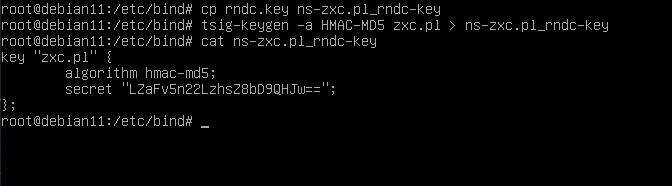
\includegraphics[width=\textwidth]{1.PNG}
            \caption{Generowanie klucza TSIG}
            \label{fig:TSIG}
        \end{figure}
        
\newpage
\section{Konfiguracja serwera DNS, rekordów RR oraz samych stref}

    \subsection{Konfiguracja pliku named.conf}
        Plik \textit{named.conf} jest głównym plikiem konfiguracyjnym serwera DNS.
        \begin{figure}[!h]
            \centering
            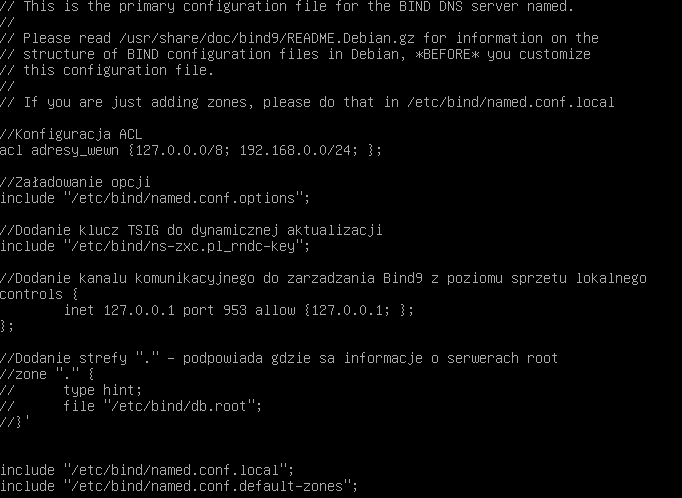
\includegraphics[width=0.9\textwidth]{2.PNG}
            \caption{Gotowy plik named.conf}
            \label{fig:named}
        \end{figure}


        W tym pliku należy wykonać poniższe czynności:
        \begin{itemize}
            \item \textbf{Konfiguracja ACL poleceniem: acl nazwa\_acl:} \\ ACL to lista adresów IP, które będą mogły podłączyć się do serwera DNS i go konfigurować.
            \item \textbf{Dodanie klucza TSIG do dynamicznej aktualizacji:} \\ Jest to załączenie pliku z kluczem TSIG przy pomocy dyrektywy \textbf{include}.
            \item \textbf{Dodanie kanału komunikacyjnego do zarządzania BIND9 z poziomu komputera lokalnego z wykorzystaniem RNDC (controls \{ ... \}):} \\ Zezwolenie na połączenie się z serwerem DNS przy pomocy RNDC z komputera o adresie 127.0.0.1 przy użyciu portu 953.
        \end{itemize}
    



    \subsection{Konfiguracja pliku named.conf.options}
    
        Plik \textit{named.conf.options} zawiera wszystkie opcje konfiguracyjne dla serwera DNS.
        \begin{figure}[h!]
            \centering
            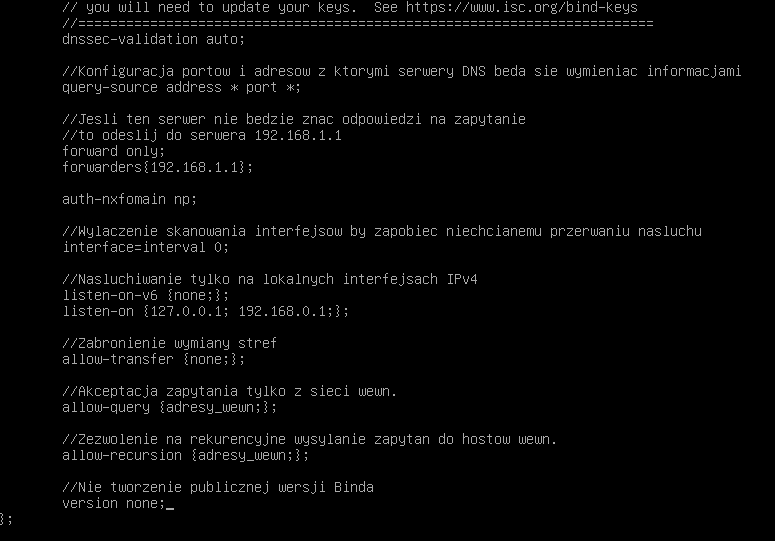
\includegraphics[width=0.93\textwidth]{3.PNG}
            \caption{Skonfigurowany plik named.conf.options}
            \label{fig:conf_opt}
        \end{figure}

        Poddane zmianom zostaną następujace aspekty:
        \begin{itemize}
            \item \textbf{Konfiguracja portów i adresów, którymi serwery DNS będą się wymieniać informacjami:} \\ Jak widać na powyższym obrazku poleceniem \textbf{query-source address * port *} zezwalamy serwerowi DNS na komunikację z serwerami o dowolnych adresach na dowolnych portach.
            \item \textbf{Konfiguracja serwera, do którego mają być przesyłane nierozwiązane zapytania:} \\ Opcje \textbf{forward only;} oraz \textbf{forwarders\{...\}} są informacją dla serwera, gdzie przesłać nierozwiązane zapytanie.
            \item \textbf{Nasłuchiwanie tylko na lokalnych interfejsach:} \\  Korzystając z poleceń \textbf{listen-on-v6: none; } oraz \textbf{listen-on \{...\}} powoduje, że serwer DNS nie będzie odpowiadał na zapytania pochodzące z adresów IPv6 oraz na zapytania przychodzące na adres inny niż wymieniony w nawiasach klamrowych.
            \item \textbf{Zablokowanie wymiany stref:} \\ Poleceniem \textbf{allow-transfer \{ none \}}; powoduje, że serwer nie będzie udostępniać informacji o strefach innym serwerom.
            \item \textbf{allow-query \{adresy\_wewn;\};:} \\ Polecenie powoduje, że zapytania do serwera DNS będą mogły pochodzić z podsieci 127.0.0.1/8 (localhost) oraz 192.168.0.0/24. Wynika to z konfiguracji pliku z obrazu \ref{fig:named}.
            \item \textbf{allow-recursion:} \\ Pozwala na wysyłanie przez serwer zapytań do hostów pochodzących z dodanych ACL.
        \end{itemize}
        
            

    \subsection{Konfiguracja pliku named.conf.local}
        Plik konfiguruje lokalne strefy DNS. W ustawieniach strefy należy dodać informację o typie strefy, o serwerach działających jako \textit{forwarder} oraz o bazach danych DNS i plikach z kluczami, które pozwalają na aktualizację wcześniej wspomnianych baz.
        \begin{figure}[!h]
            \centering
            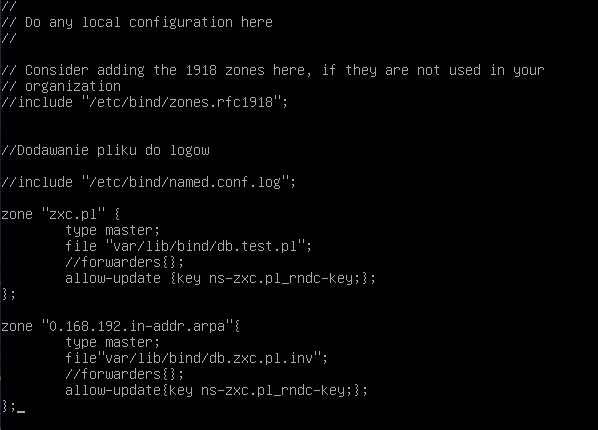
\includegraphics[width=0.93\textwidth]{4.PNG}
            \caption{Skonfigurowany plik named.conf.local}
            \label{fig:named_conf_local}
        \end{figure}

\pagebreak

        Dodać do pliku trzeba dwie zależności:
        \begin{itemize}
            \item \textbf{zone ''zxc.pl'':} \\ W ten sposób została dodana strefa zxc.pl. Jej typ to \textit{master}, a klucz, który zezwala na aktualizację tej strefy znajduje się w pliku \\ \textbf{''ns-zxc.pl\_rndc-key'';}. Plik z rekordami RR tej strefy ustawiony paramterem \textbf{file} to \textbf{"/var/lib/bind/db.zxc.pl"}.
            \item \textbf{zone 0.168.192.in-addr.arpa:} \\ W ten sposób dodaje się strefę ARPA (czyli odwrotny DNS). Tak jak wcześniej dodana strefa zxc.pl strefa ARPA jest typu master, jej plik z rekordami RR to \textbf{"/var/lib/bind/db.zxc.pl.inv";}. Nie posiada ona żadnych serwerów działających jako \textit{forwarderzy}. Klucz umożliwiający aktualizację strefy to plik \textbf{''ns-zxc.pl\_rndc-key'';}.
        \end{itemize}
            

    \subsection{Konfiguracja rekordów \textit{Resource Records}}
        \begin{figure}[!h]
            \centering
            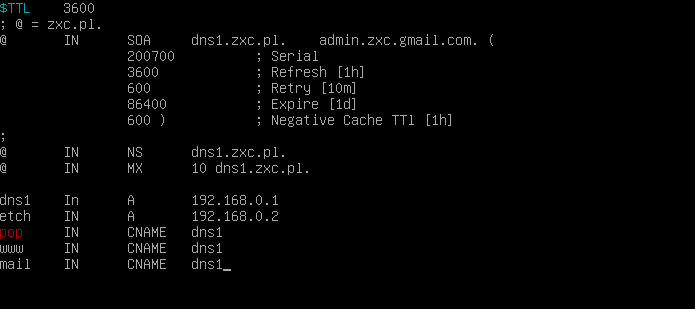
\includegraphics[width = 1.05\textwidth]{5.PNG}
            \caption{Rekordy RR dla strefy zxc.pl}
            \label{fig:testpl}
        \end{figure}
        \newpage
        \begin{figure}[!h]
            \centering
            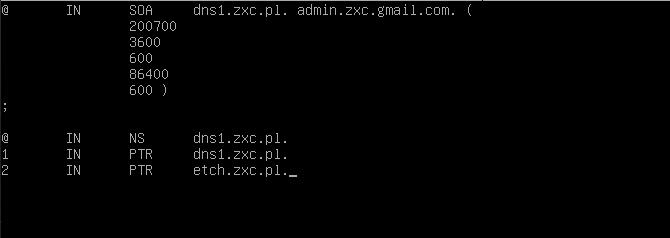
\includegraphics[width = \textwidth]{6.PNG}
            \caption{Rekordy RR dla strefy 0.168.192.in-addr.arpa}
            \label{fig:arpa}
        \end{figure}

        \subsubsection{Co to są rekordy RR?}
            Rekordy RR oznaczają jaki typ informacji przechowuje dana strefa DNS. Każdy rekord ma swój typ, czas, po którym wygasa oraz informacje specyficzne dla samego siebie.
            
        \subsubsection{Rodzaje rekordów RR}

        \begin{itemize}
            \item \textbf{SOA - Start of authority record:} \\ Rekord ten przechowuje autorytatywne informacje o strefie DNS, włączając w to główny serwer rozpoznawania nazw, email administratora, numer seryjny strefy oraz kilka liczników czasu, które powiązane są z odświeżaniem informacji o strefie. Liczniki te są informacjami dla serwerów zapasowych, które mają synchronizować się z głównym serwerem.
            \item \textbf{Rekord NS:} \\  Informacja dla serwera DNS o adresach pozostałych serwerów. Rekordy te mają wskazywać na rekordy typu A, które należy utworzyć w pliku.
            \item \textbf{Rekord A:} \\ Rekord używany do mapowania nazw na adresy.
            \item \textbf{Rekord CNAME:} \\ Rekord ten jest rozszerzeniem rekordu A, czyli przekierowuje ``nazwe2 na nazwe1``, gdzie nazwa1 jest wcześniej nakierowana np. na adres 192.168.0.1.
            \item \textbf{Rekord MX:} \\ Rekord \textit{Mail Exchange} powstały na potrzeby usługi poczty elektronicznej. Przy pomocy tego rekordu oznacza się serwery poczty. Tak jak rekord NS, rekord MX musi być nakierowany na nazwę, która jest rozwiązana rekordem typu A.
            \item \textbf{Rekord PTR:} \\ Rekord mapujący adres IP na nazwę hosta. Używa się go w zapytaniach typu \textit{reverse DNS}
        \end{itemize}
        
        
\newpage

    \subsection{Test za użyciem narzędzia dig}
        \begin{figure}[!h]
            \centering
            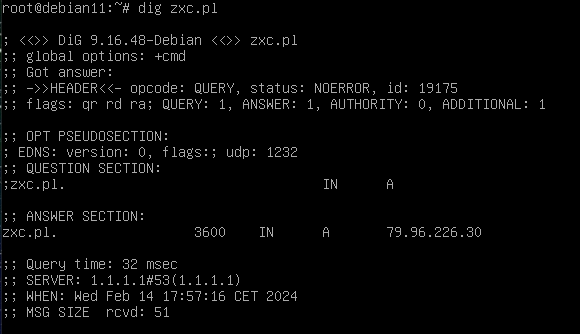
\includegraphics[width=0.95\textwidth]{7.PNG}
            \caption{Wynik komendy Dig dla domenty zxc.pl}
            \label{fig:dig1}
        \end{figure}
        \begin{figure}[!h]
            \centering
            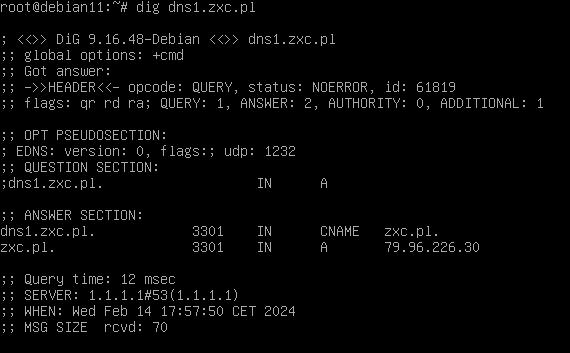
\includegraphics[width=0.95\textwidth]{8.PNG}
            \caption{Wynik komendy Dig dla dns1.zxc.pl}
            \label{fig:dig2}
        \end{figure}
        Jak widać domena zwraca odpowiednie wartości rekordów, jeżeli zostanie ``wypytana`` przez narzędzie \textit{dig}. 

\end{document}